\documentclass[a4paper,12pt]{article} 

%%% Работа с русским языком
\usepackage{cmap}                           % поиск в PDF
\usepackage{mathtext} 			 	       % русские буквы в формулах
\usepackage[T2A]{fontenc}               % кодировка
\usepackage[utf8]{inputenc}              % кодировка исходного текста
\usepackage[english,russian]{babel}  % локализация и переносы
\usepackage[left=2cm,right=2cm,
    top=2cm,bottom=3cm,bindingoffset=0cm]{geometry}
\usepackage{wrapfig}
\usepackage{gensymb}
\usepackage{textcomp}
\usepackage{multirow}
\usepackage{amsmath,amsfonts,amssymb,amsthm,mathtools} % AMS
\usepackage{euscript}	 % Шрифт Евклид
\usepackage{mathrsfs} % Красивый матшрифт
\usepackage{graphicx}%Вставка картинок правильная
\usepackage{float}%"Плавающие" картинки
\usepackage{wrapfig}%Обтекание фигур (таблиц, картинок и прочего)
\title{Лабораторная работа 3.3.2

Закон трёх вторых}
\author{Кагарманов Радмир Б01-106}
\date{28 ноября 2022 г.}

\begin{document}
\maketitle
\thispagestyle{empty}
\newpage
\setcounter{page}{1}

\paragraph{Цель работы:} исследовать вольт-амперные характеристики диода при различных токах накала и по результатам измерений определить удельный заряд электрона.

\paragraph{В работе используется:} радиолампа с цилиндрическим анодом; стабилизированные источники постоянного тока и постоянного напряжения; мультиметр-амперметр. 

\paragraph{Экспериментальная установка\\}
Исследования проводятся на диоде 2Ц2С с косвенным накалом. Радиус его катода $r_{к} = 0,9 ~мм$, радиус анода $r_{а} = 9,5 ~мм$, коэффициент $\beta^2 = 0,98$. Полная высота анода и катода составляет около 20 мм, однако эмиссия электронов происходит только с центральной части катода, покрытой оксидным слоем. Высота этого слоя $l = 9~мм$. Поскольку рабочая часть достаточно удалена от его торцов, электрическое поле в этой части с хорошей точностью можно считать радиальным. \par

\begin{figure}[!h]
\centering
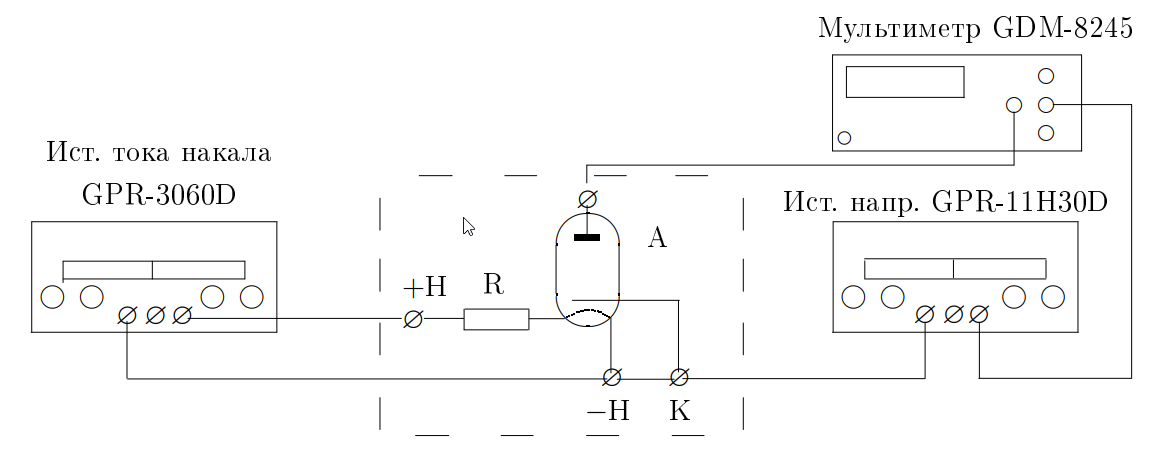
\includegraphics[width=0.9\linewidth]{экспериментальная установка.png}
\caption{Экспериментальная установка}
\label{fig:mpr}
\end{figure}

Схема экспериментальной установки изображена на рис. 1. Для подогрева катода и для питания анода используются стабилизированные источники постоянного тока и напряжения. В цепь накала включено предохранительное сопротивление $R$. Анодное напряжение измеряется вольтметром источника питания, анодный ток - многопредельным мультиметром.

\paragraph{Обработка результатов:}

\subparagraph{1.} Построим графики зависимости $I_а=f(V_{а}^{3/2})$. По наклону прямолинейных участков вычислим $e/m$ электрона. На рисунках 2-5 будут изображены эти графики для различных токов накала.

\newpage

\begin{figure}[!h]
\centering
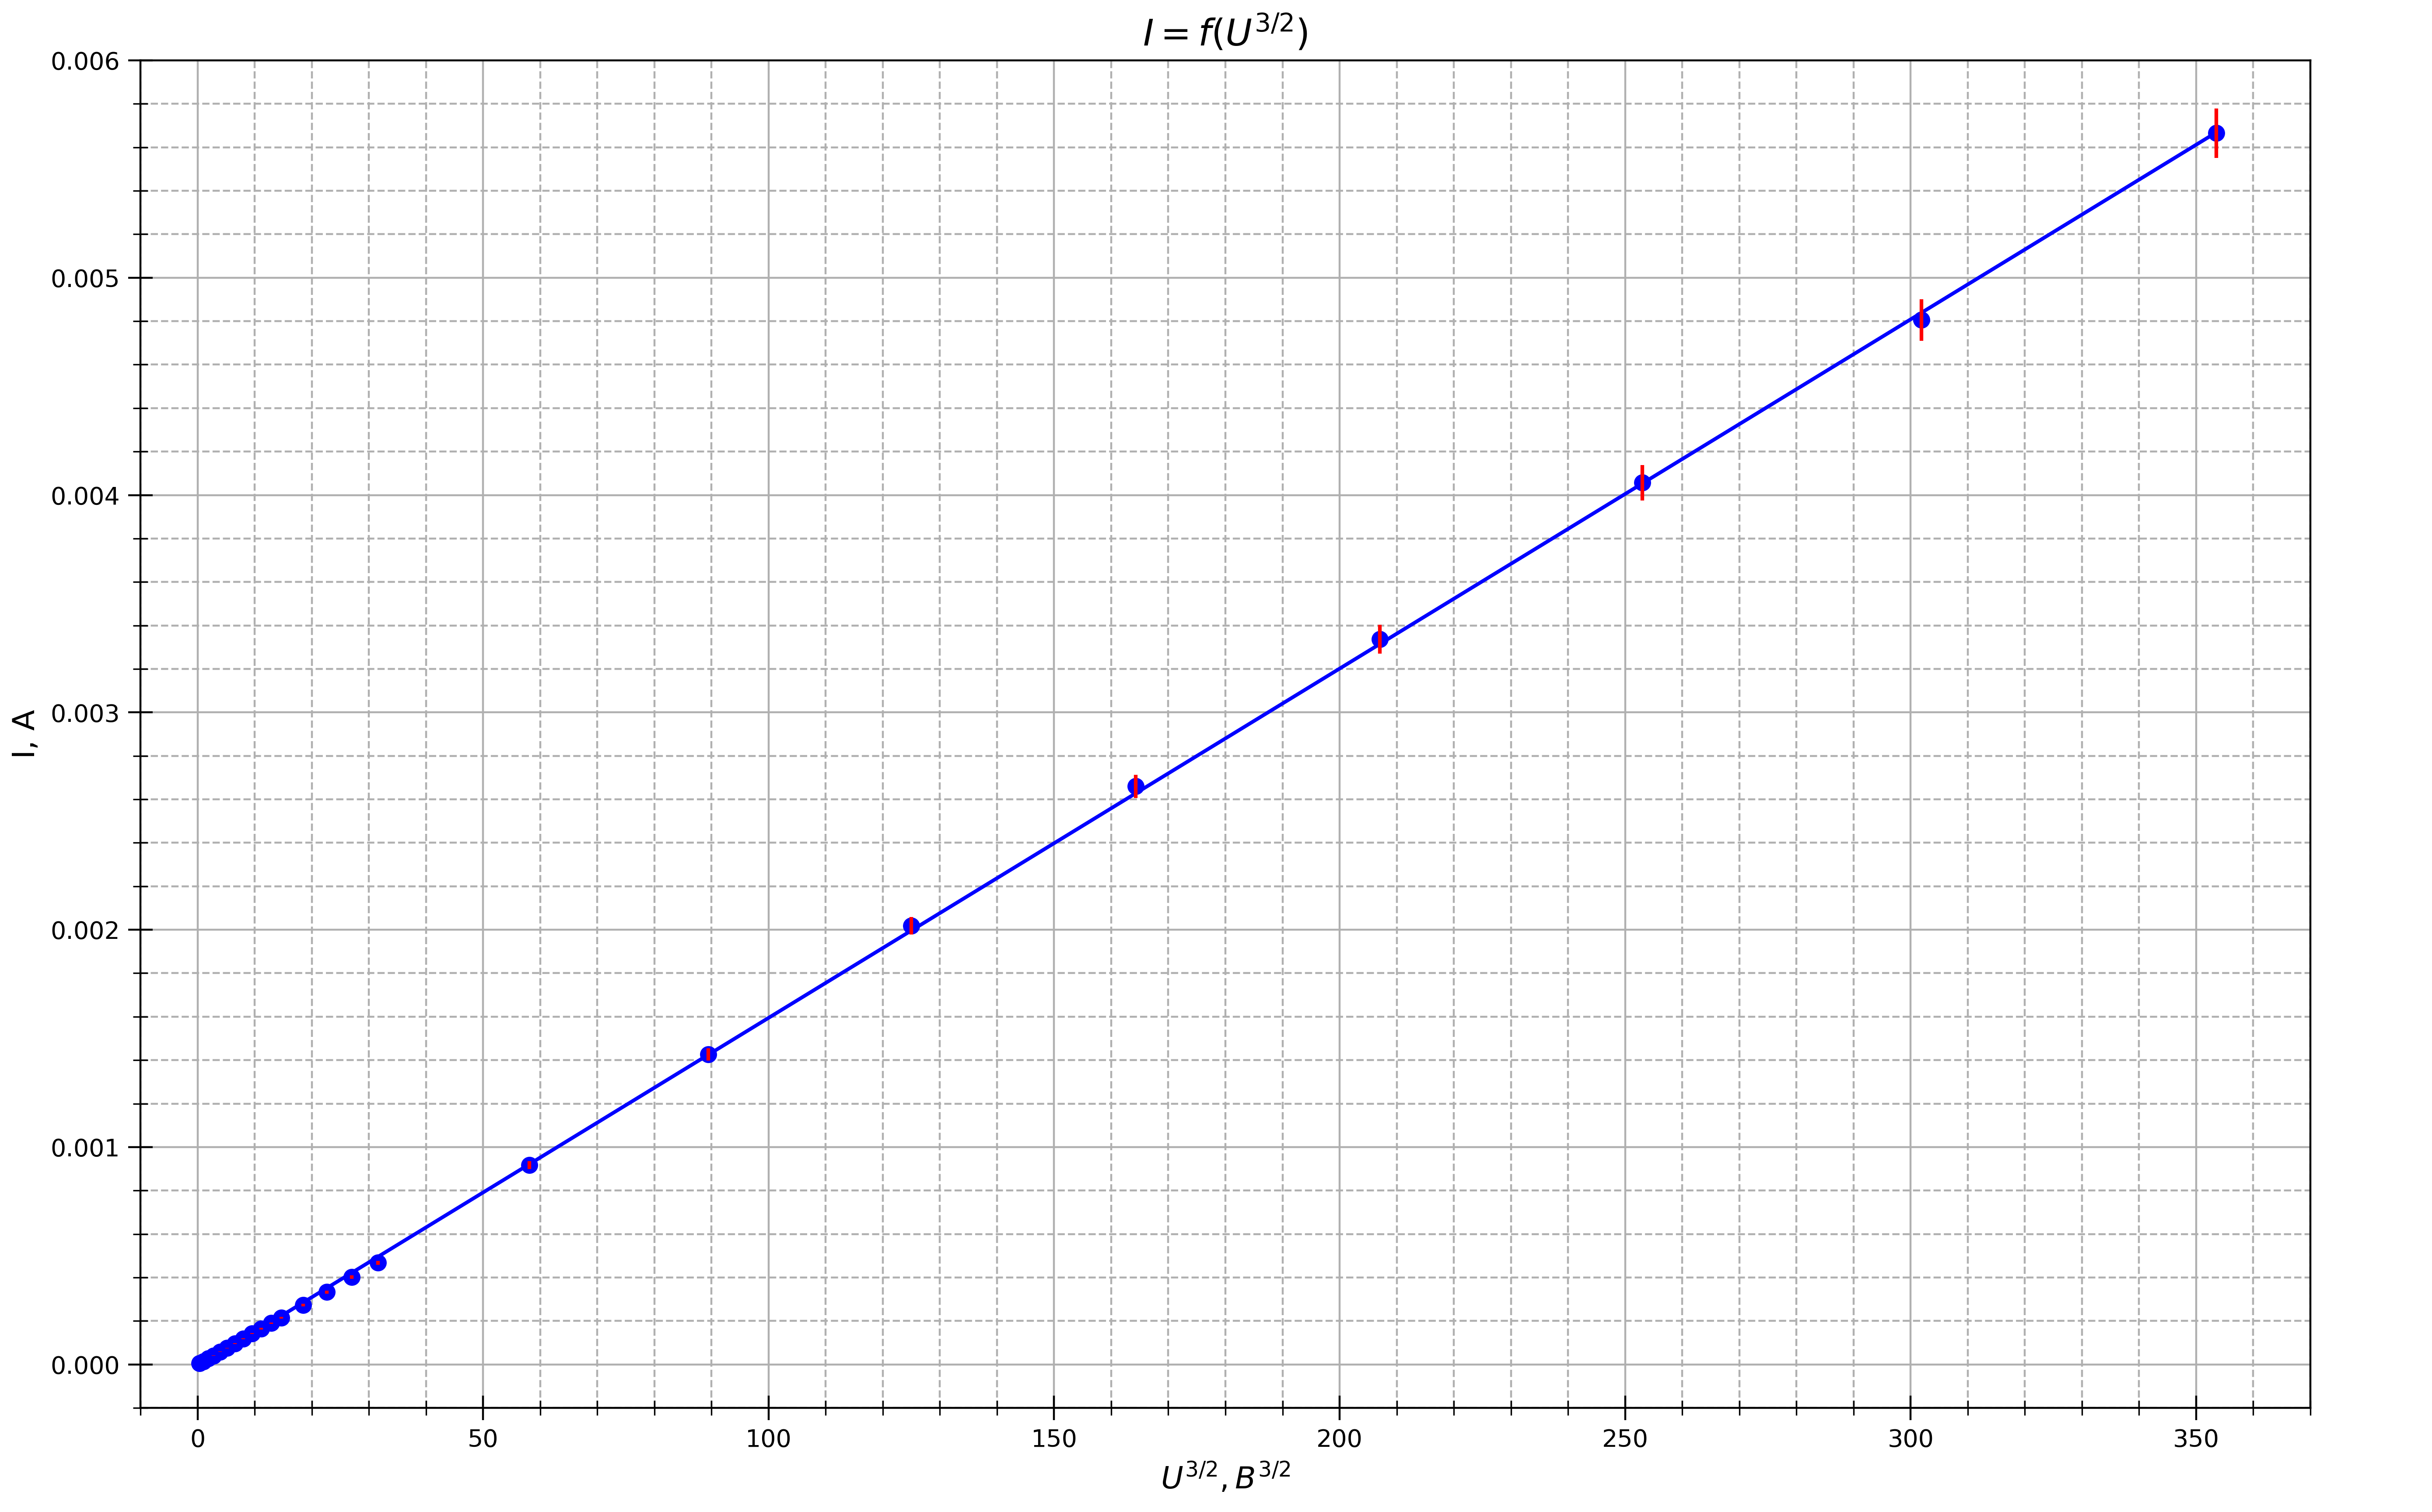
\includegraphics[width=0.9\linewidth]{I=1,3.png}
\caption{$I_{н}=1,3~А$}
\label{fig:mpr}
\end{figure}

\begin{figure}[!h]
\centering
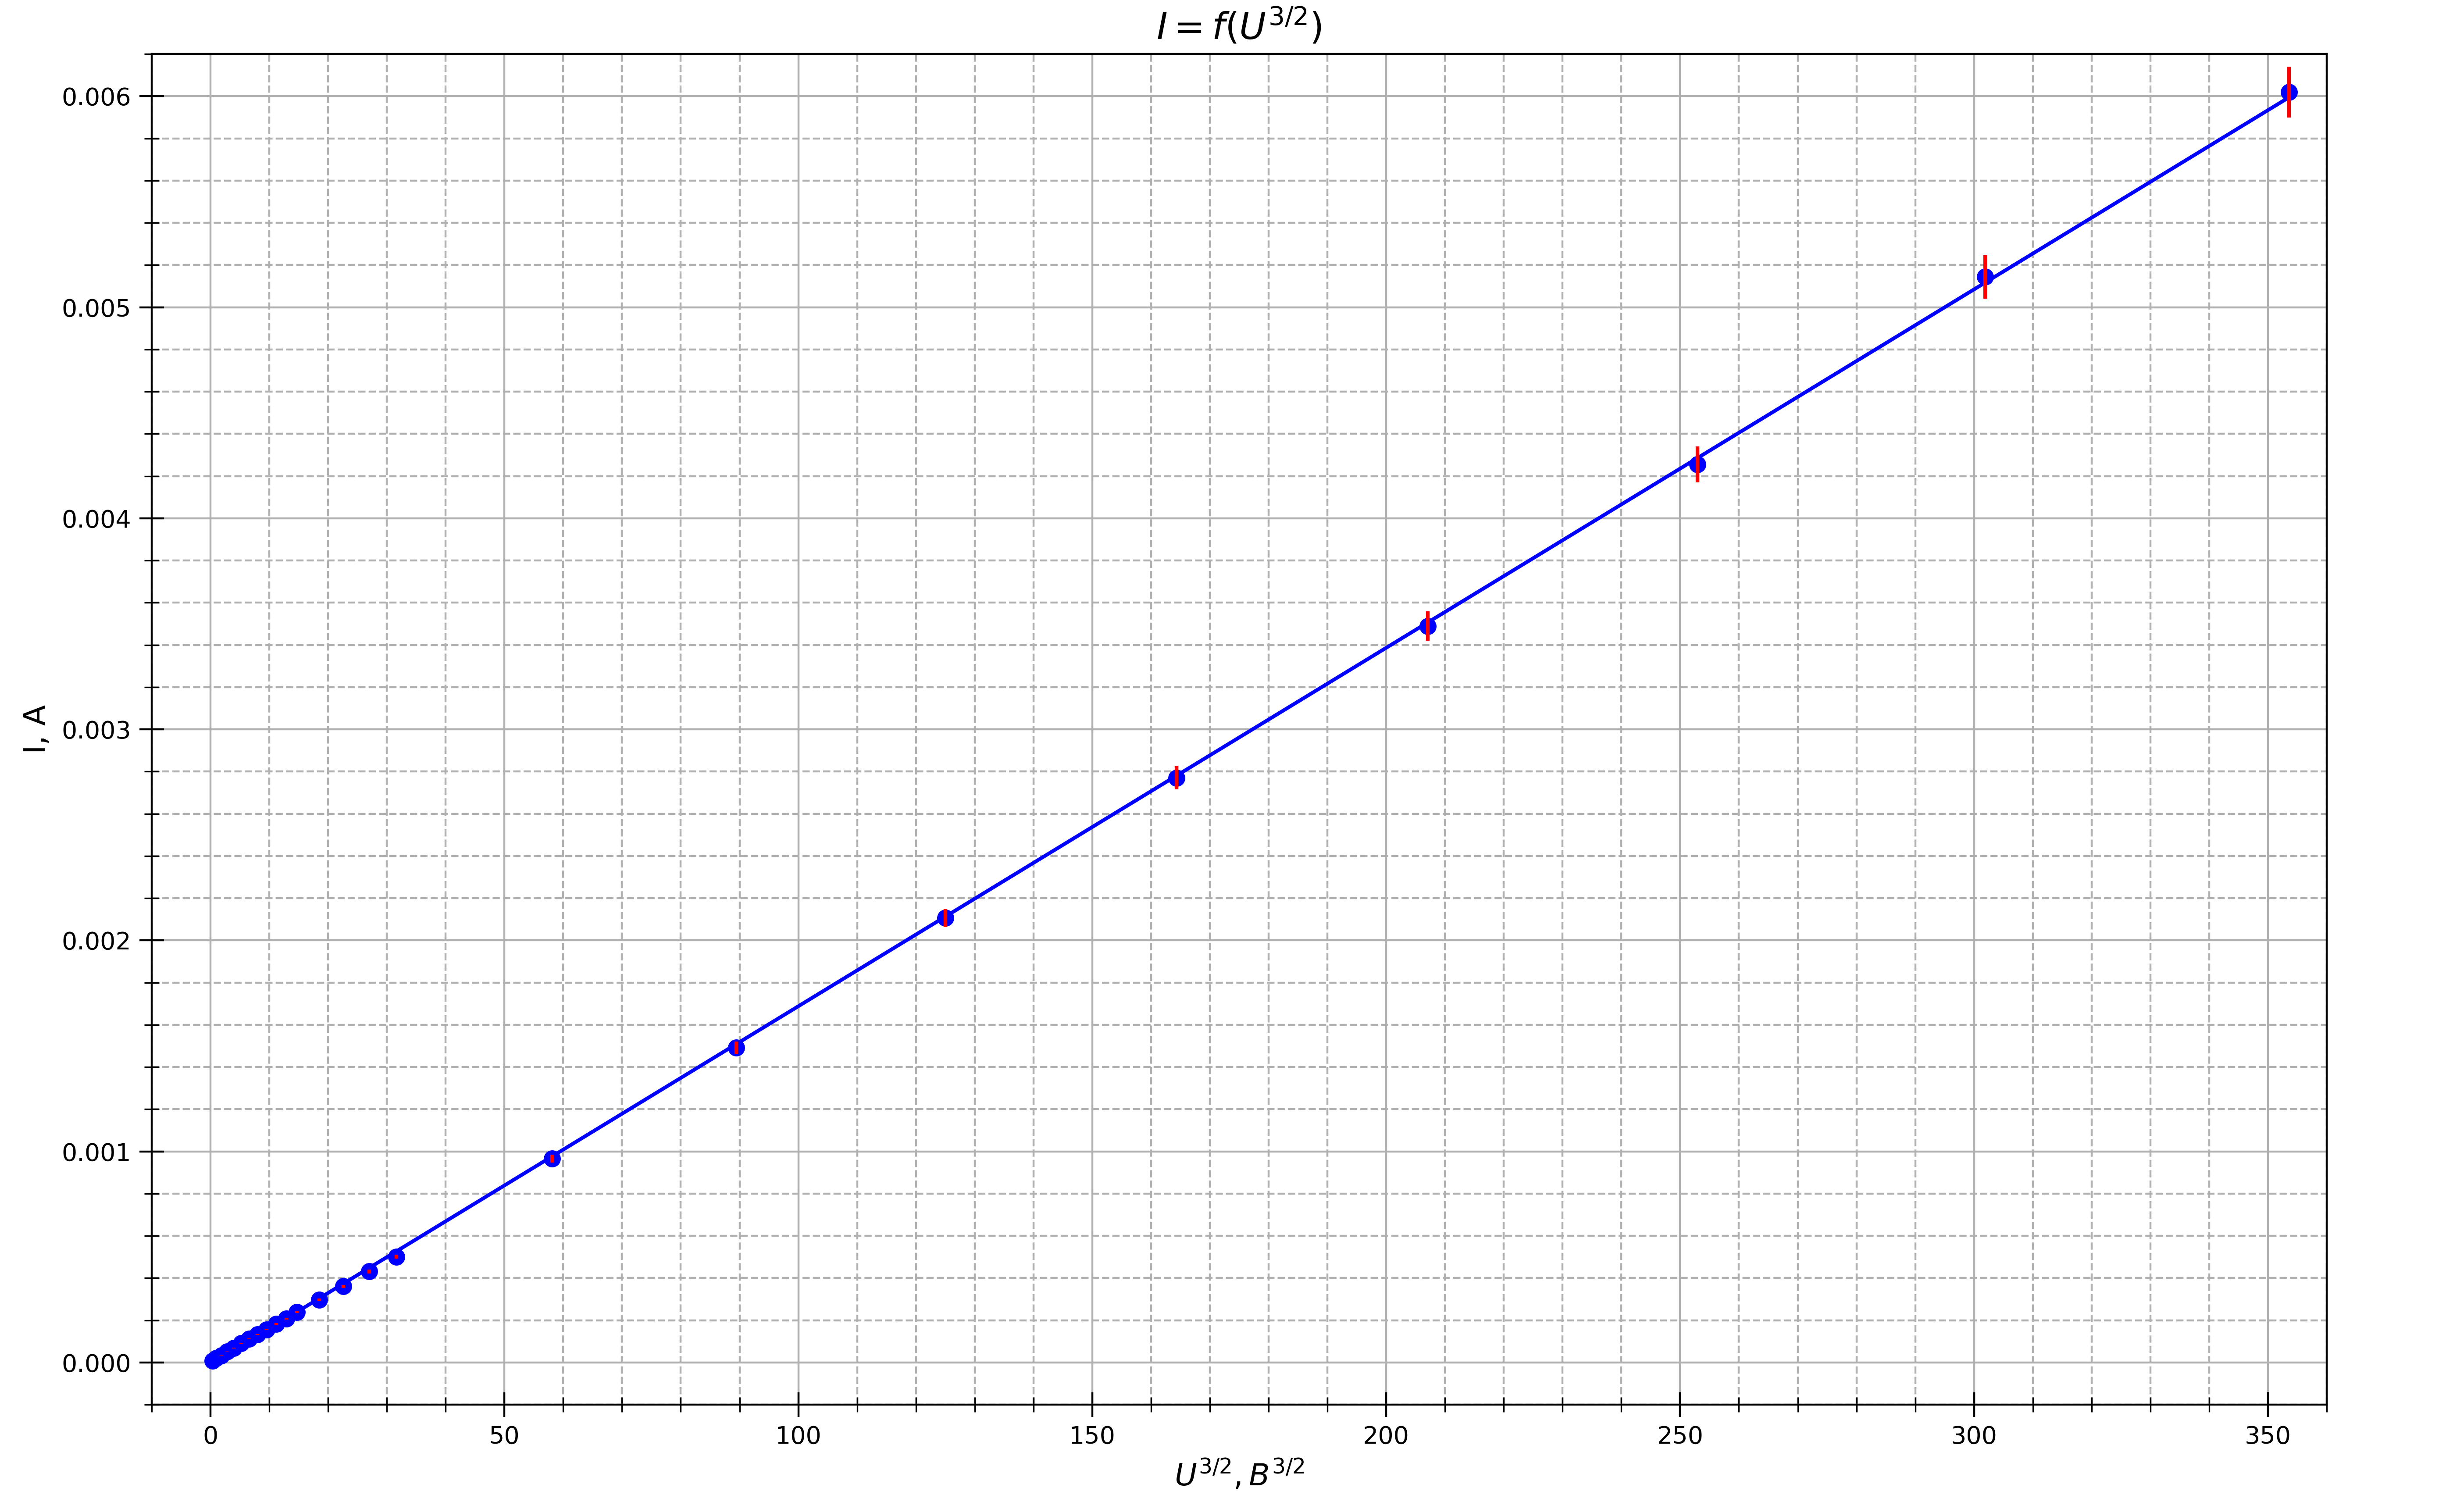
\includegraphics[width=0.9\linewidth]{I=1,4.png}
\caption{$I_{н}=1,4~А$}
\label{fig:mpr}
\end{figure}

\newpage

\begin{figure}[!h]
\centering
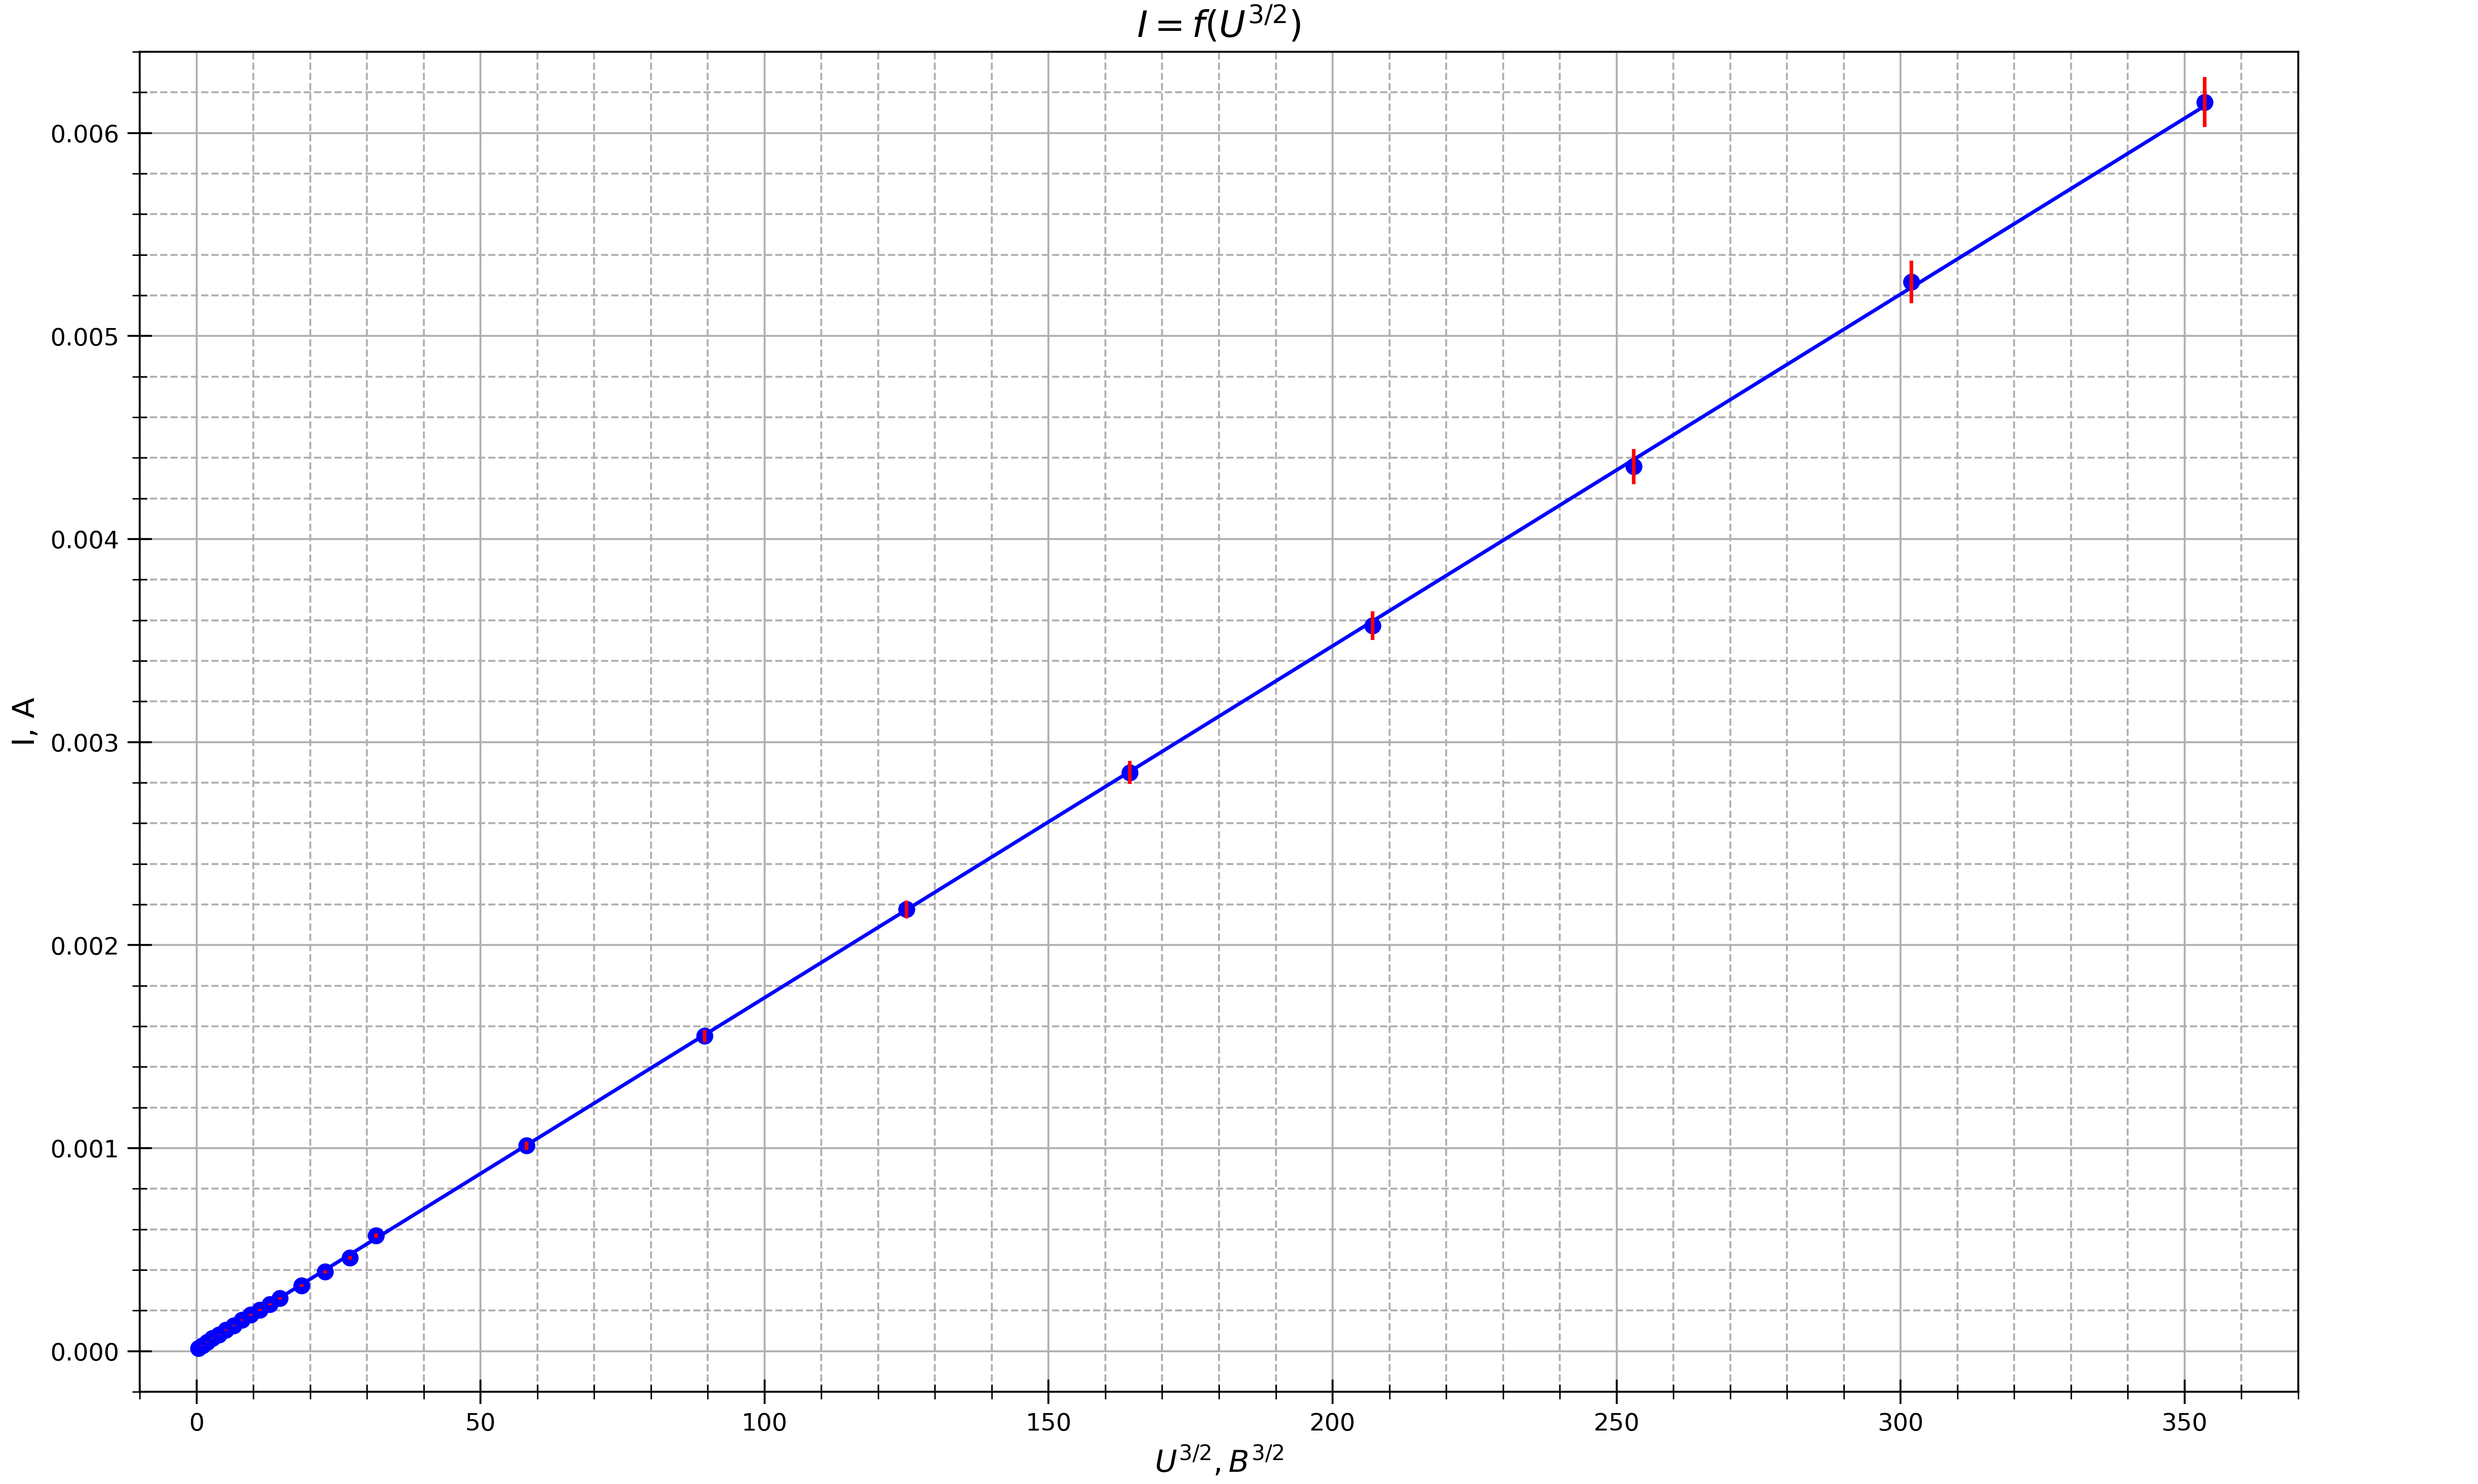
\includegraphics[width=0.9\linewidth]{I=1,5.png}
\caption{$I_{н}=1,5~А$}
\label{fig:mpr}
\end{figure}

\begin{figure}[!h]
\centering
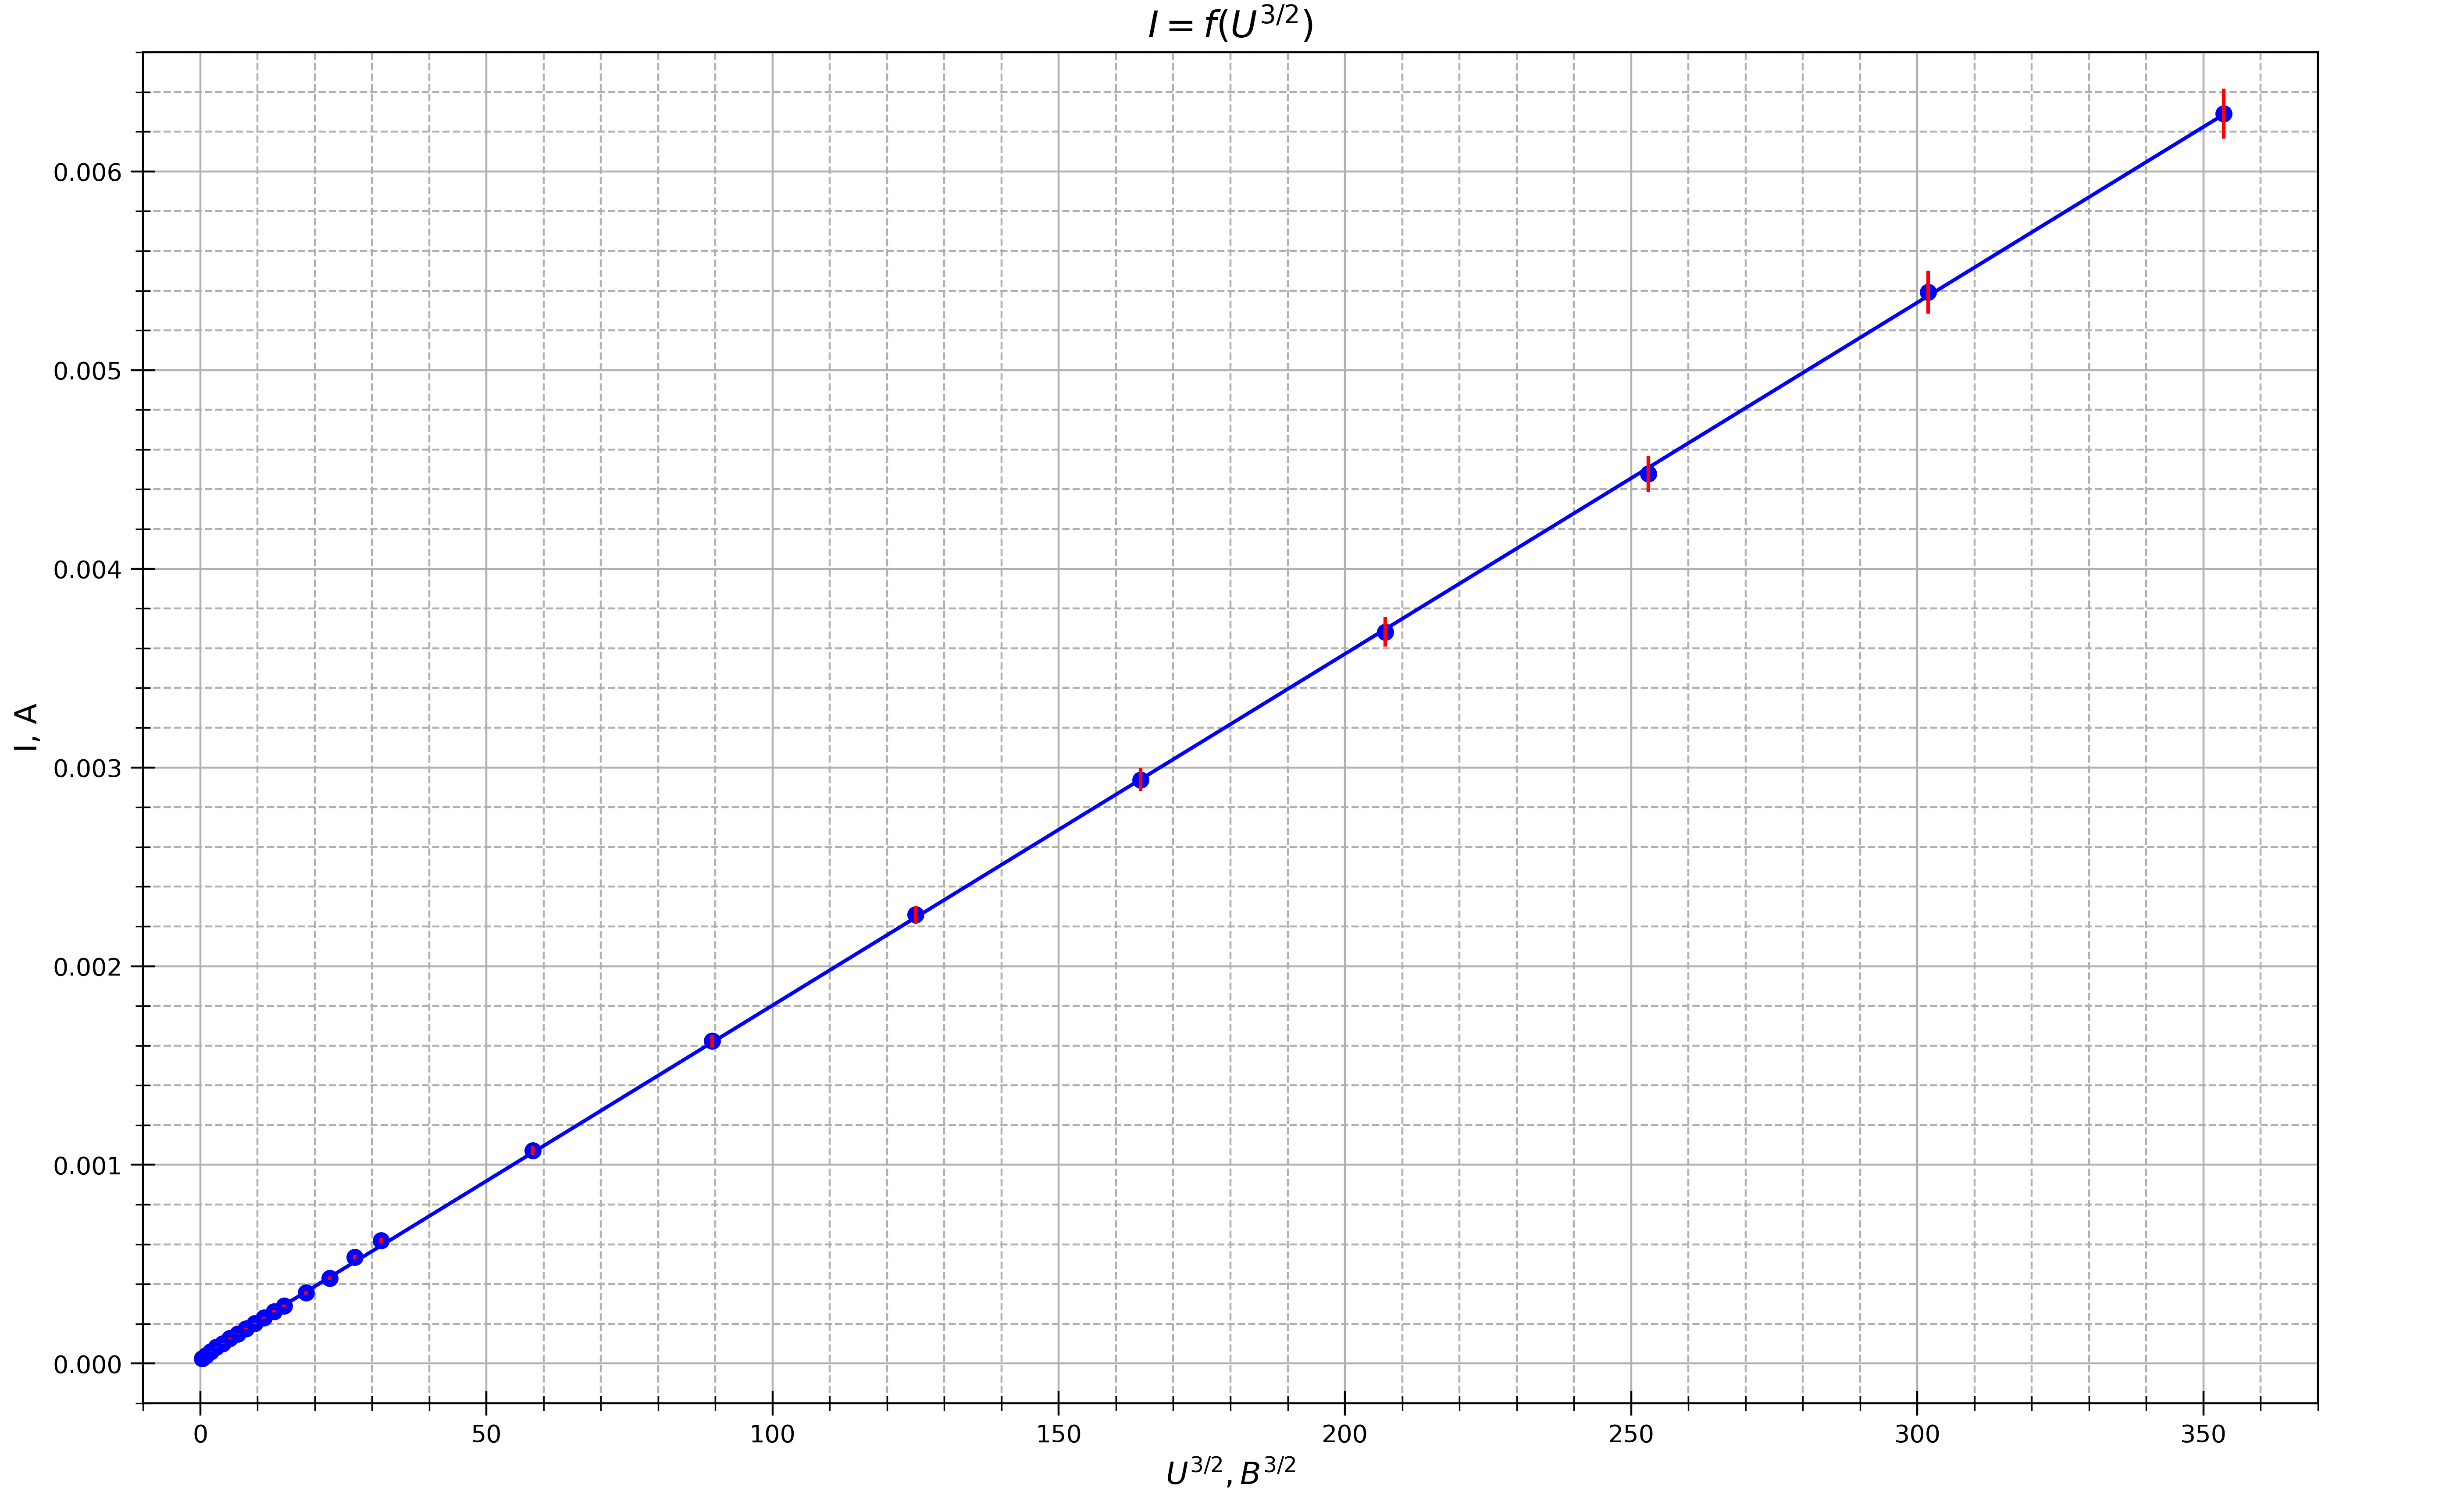
\includegraphics[width=0.9\linewidth]{I=1,6.png}
\caption{$I_{н}=1,6~А$}
\label{fig:mpr}
\end{figure}

Исследуемый закон может быть представлен следующим образом:
\begin{equation}
    I=\alpha A_0 U^{3/2},
\end{equation}

где $\alpha$ - функция отношения $r_{а}/r_{к}$(т.к. $r_{а}/r_{к}\approx 10$, то $\alpha = 1.05$), а $A_0 = \frac{4}{9}\varepsilon_0 \frac{2\pi l}{r_{а}}\sqrt{\frac{2e}{m}}$. 
\newpage
Отсюда находим $e/m$:
\begin{center}
    $I_{н}=1,3~А:~\frac{e}{m}=2,14\cdot 10^{11}~\frac{Кл}{кг}$\\ 
    $I_{н}=1,4~А:~\frac{e}{m}=2,39\cdot 10^{11}~\frac{Кл}{кг}$\\
    $I_{н}=1,5~А:~\frac{e}{m}=2,49\cdot 10^{11}~\frac{Кл}{кг}$\\
    $I_{н}=1,6~А:~\frac{e}{m}=2,59\cdot 10^{11}~\frac{Кл}{кг}$\\
\end{center}
Из результатов видно, что ток накала влияет на значение удельного заряда.

\subparagraph{2.}Построим графики в тех координатах, но со значениями до 10 В. На рисунках 6-7 можно увидеть, что зависимость линейная.

\paragraph{Вывод:} мы исследовали вольт-амперные характеристики диода при различных токах накала и по результатам измерений определили удельный заряд электрона.

\newpage
\begin{figure}[!h]
\centering
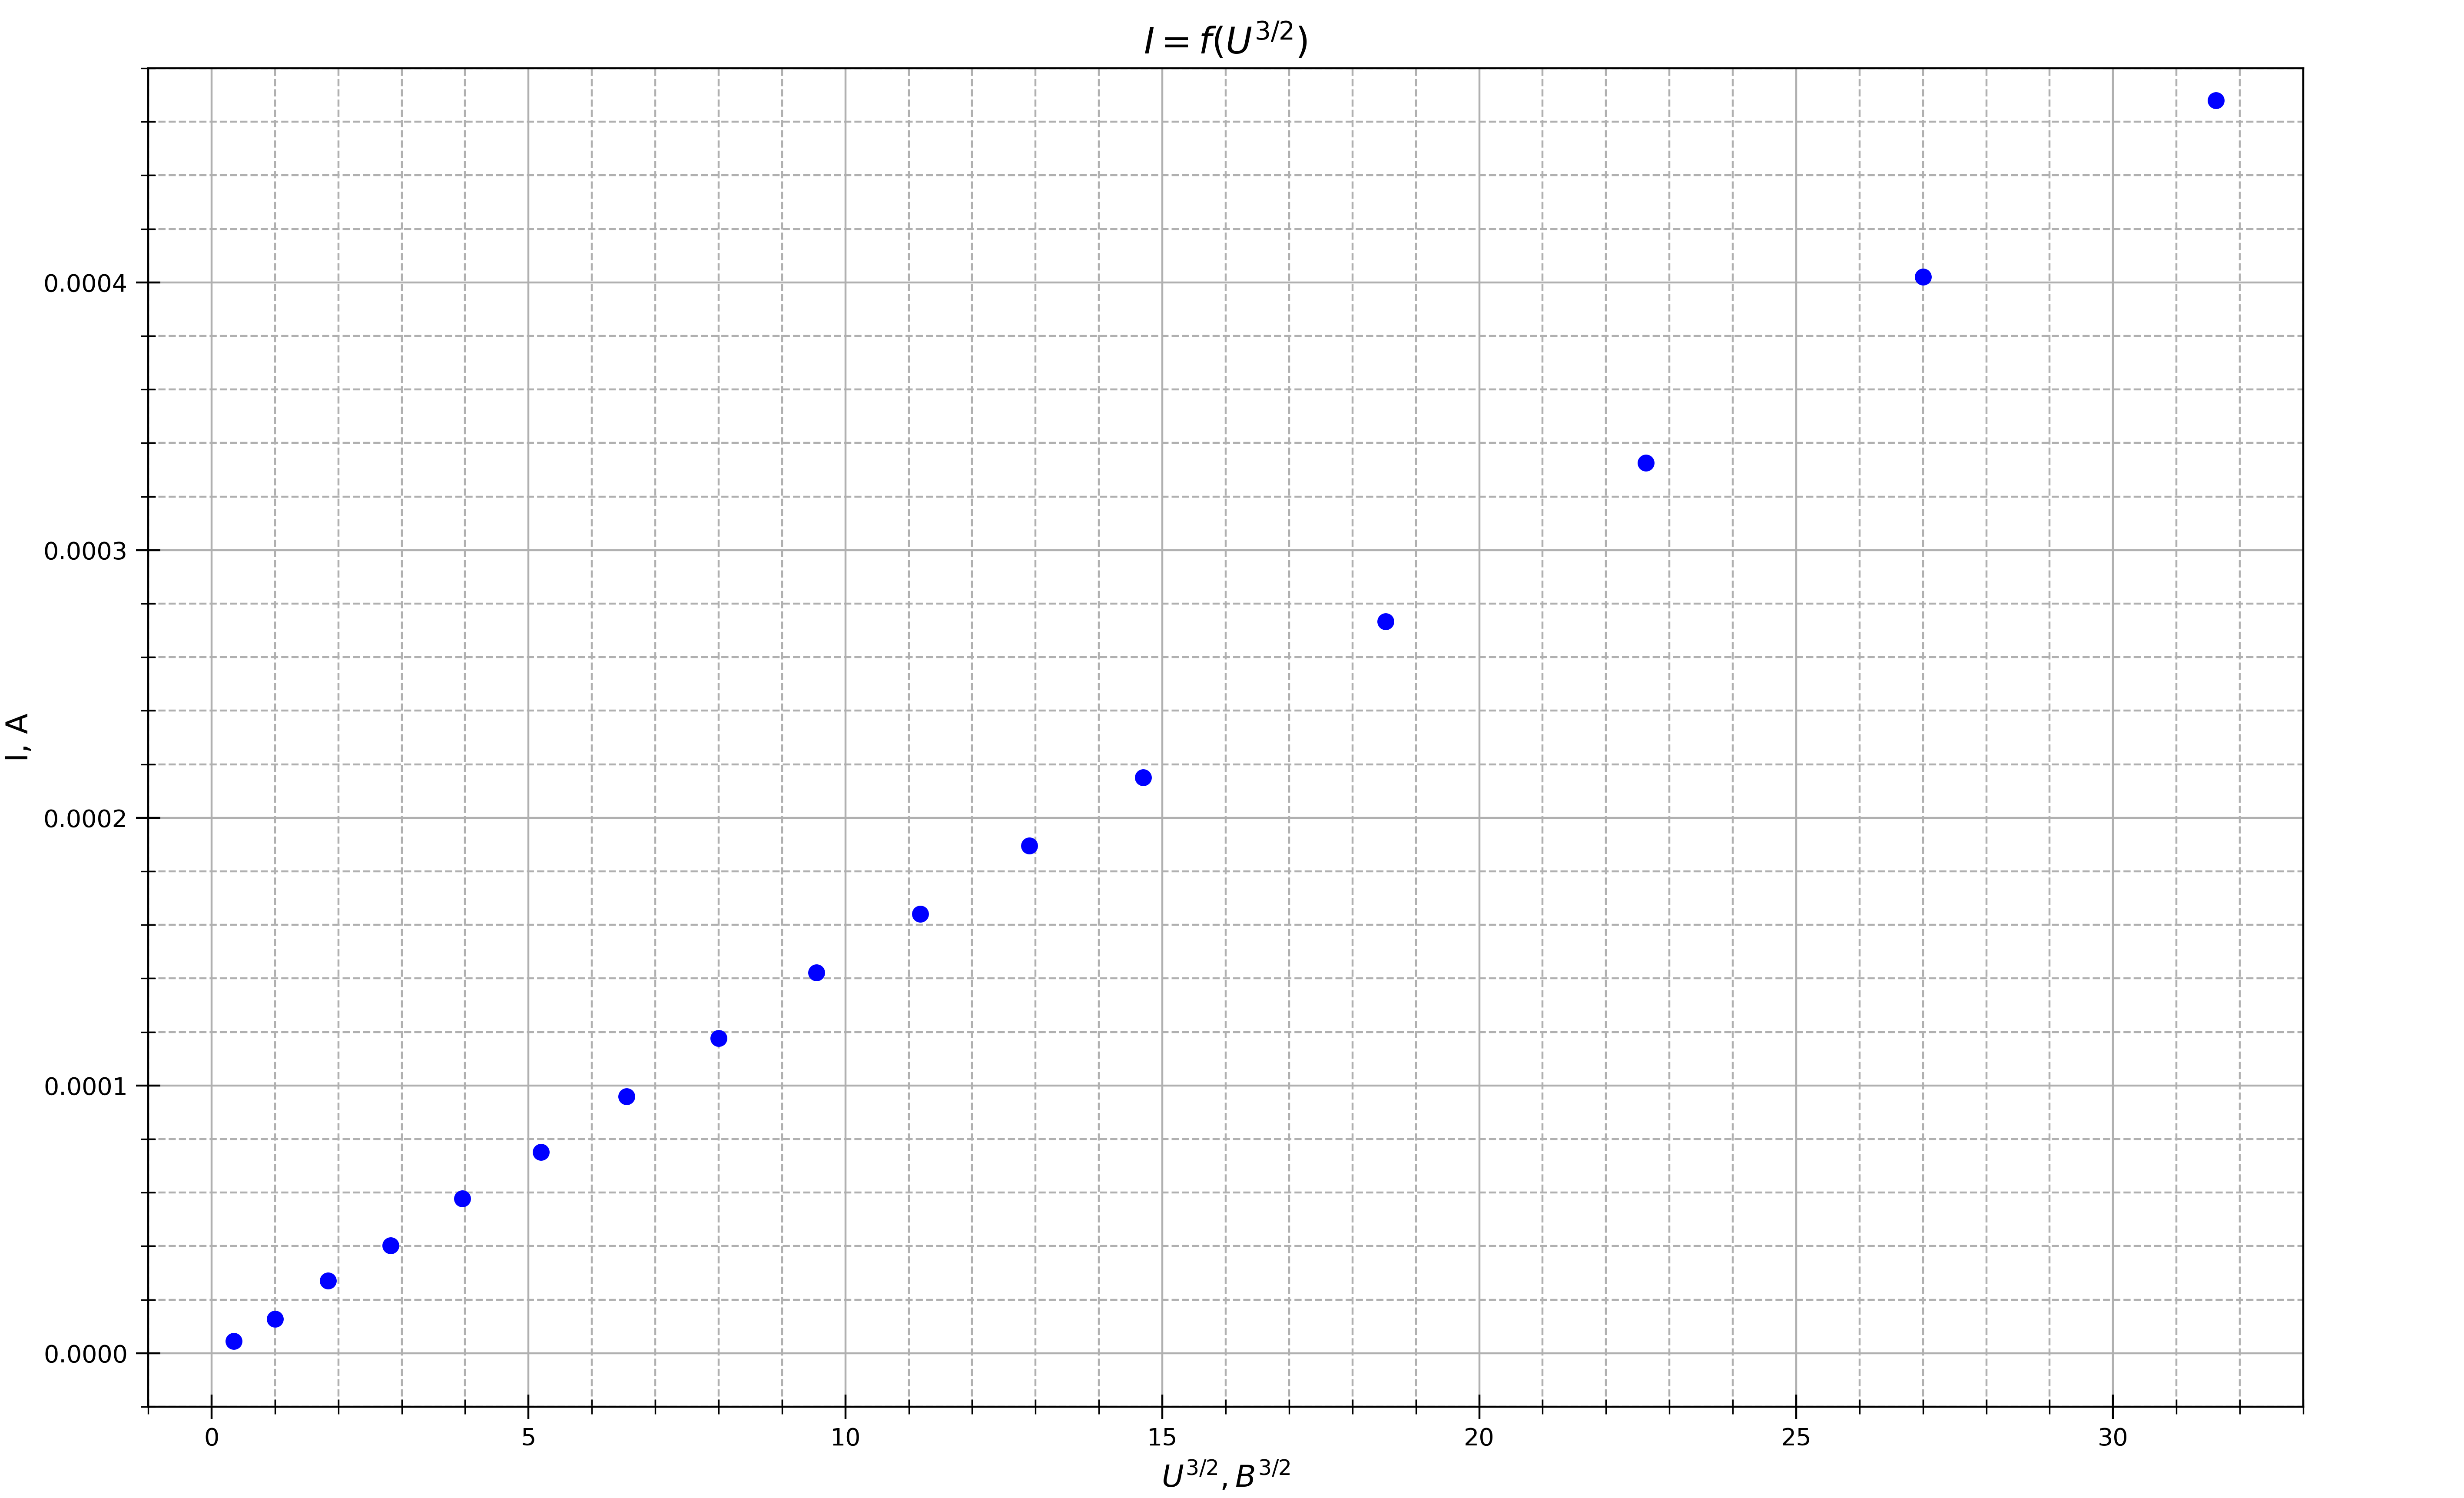
\includegraphics[width=0.9\linewidth]{VI=1,3.png}
\caption{$I_{н}=1,3~А$}
\label{fig:mpr}
\end{figure}
\begin{figure}[!h]
\centering
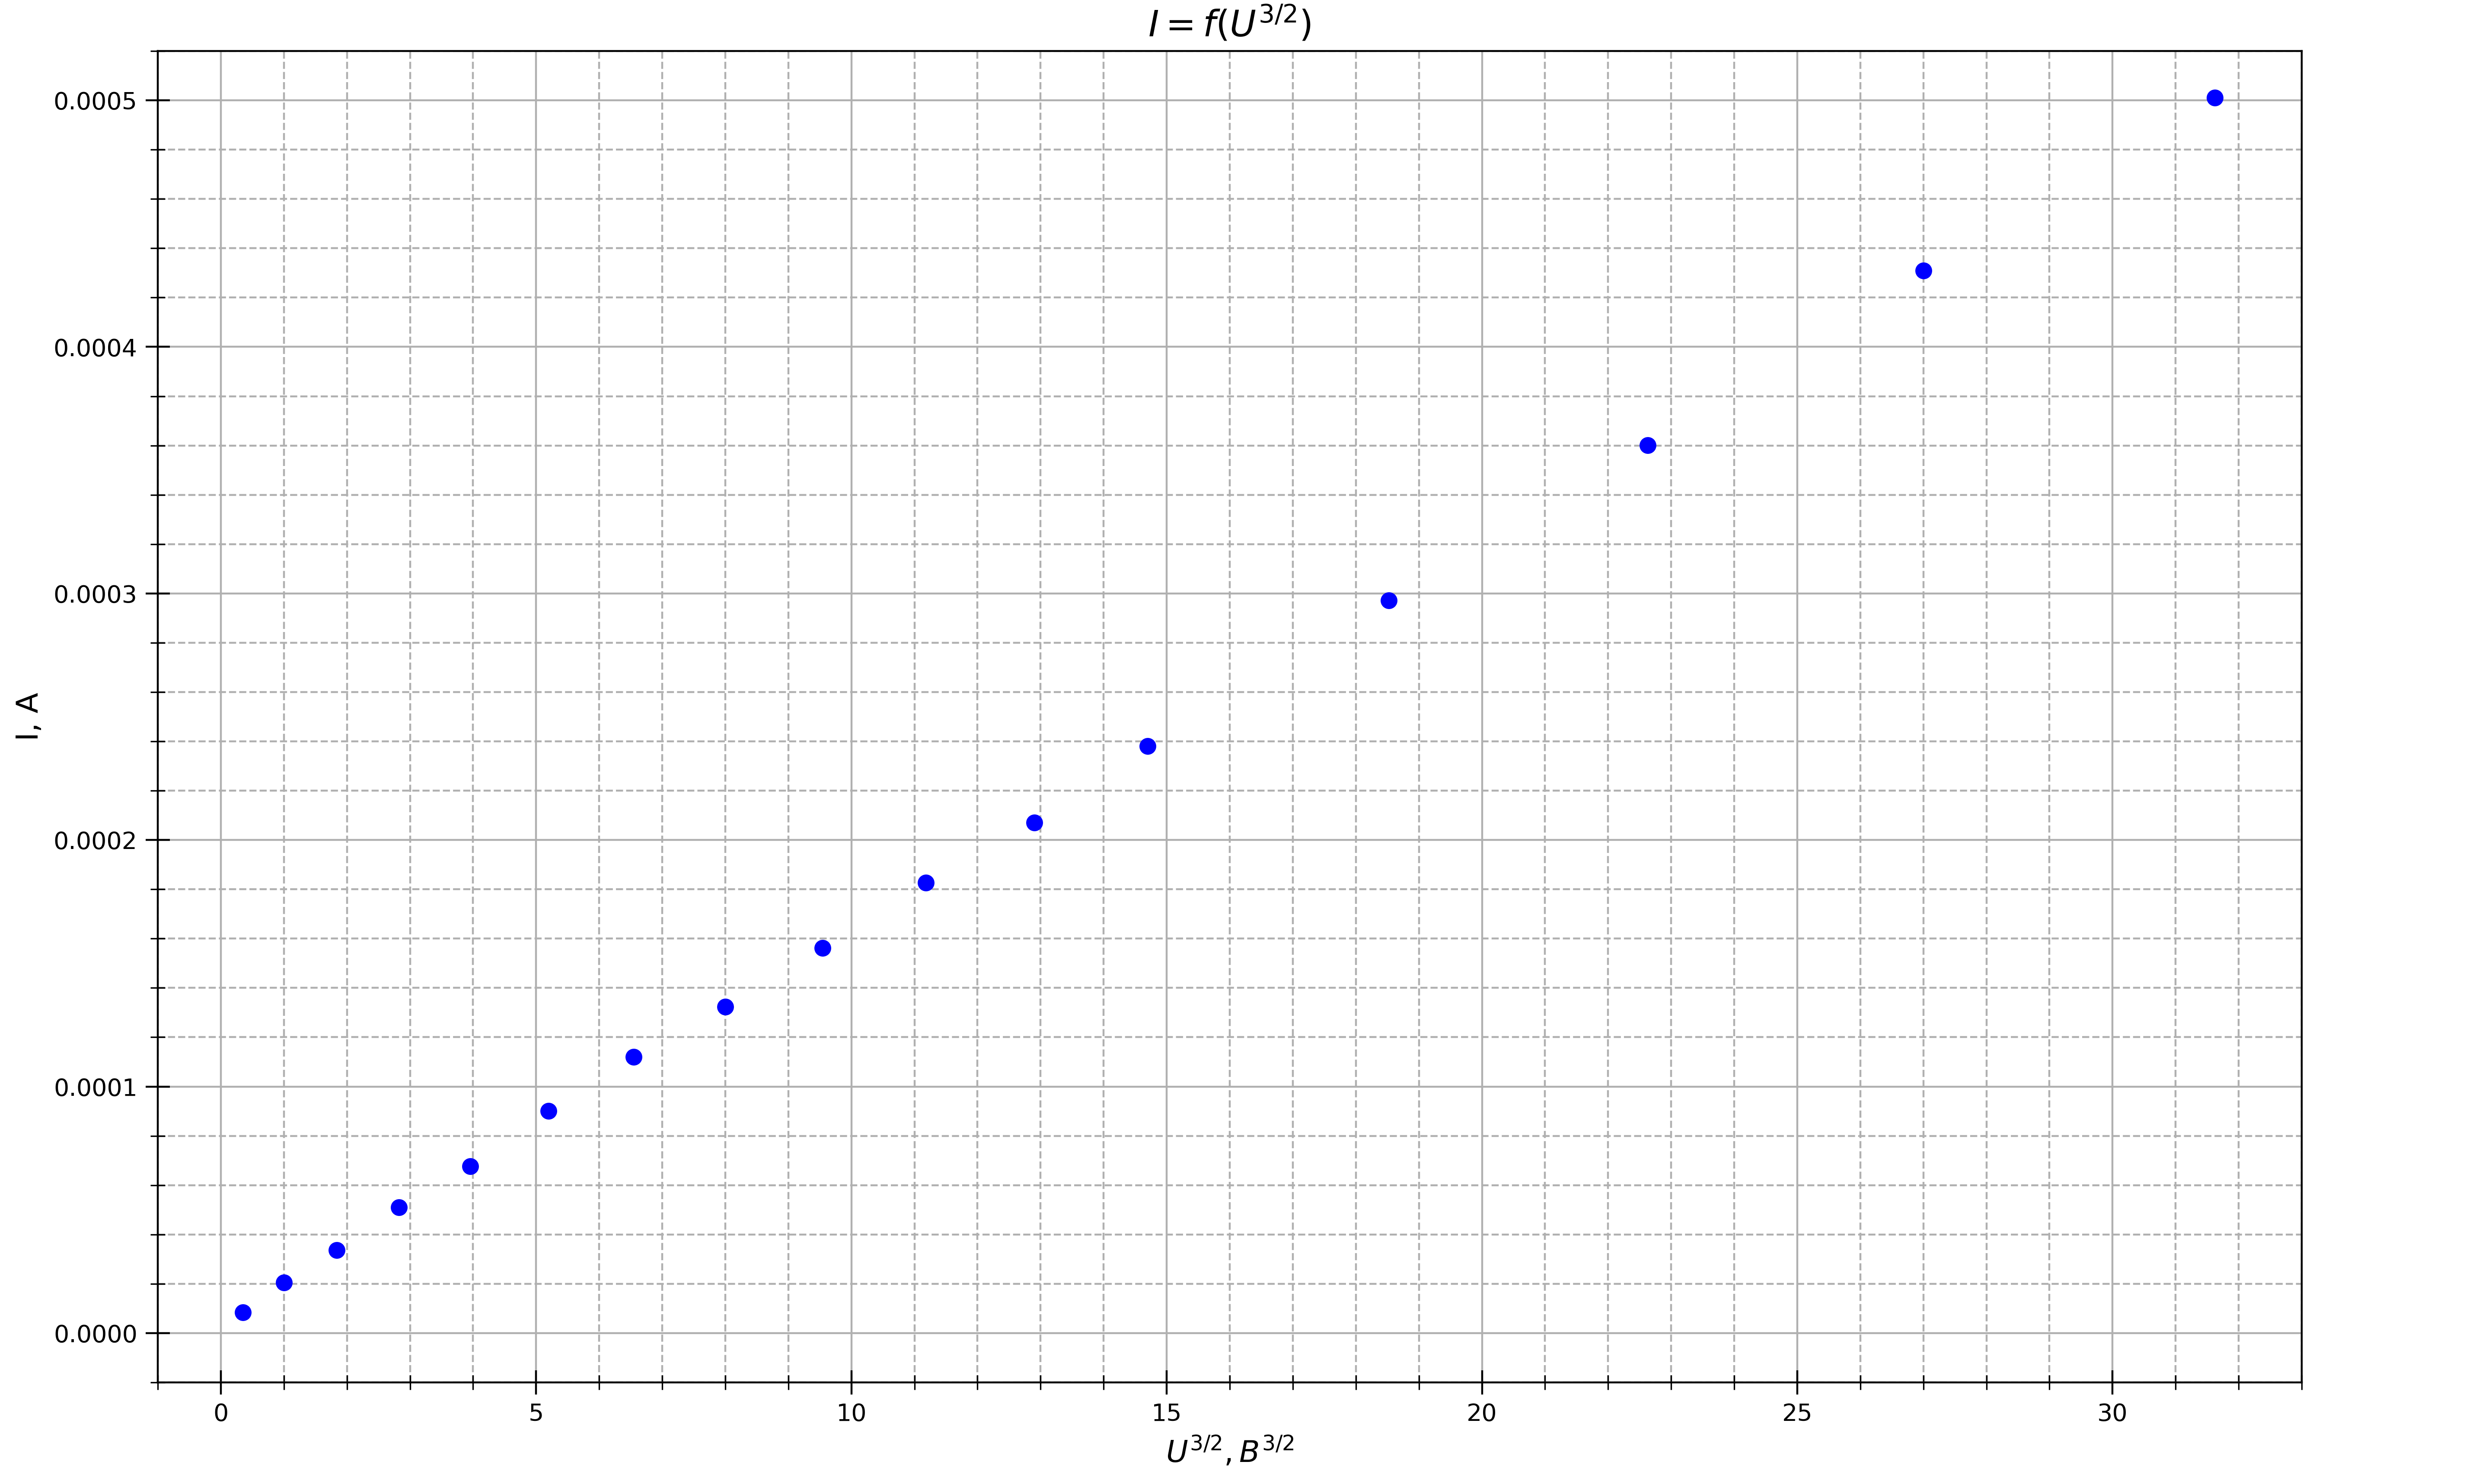
\includegraphics[width=0.9\linewidth]{VI=1,4.png}
\caption{$I_{н}=1,4~А$}
\label{fig:mpr}
\end{figure}

\end{document}
